\documentclass[a4paper,11pt]{article}
\usepackage[utf8]{inputenc}	% character encoding
\usepackage{amsmath,amssymb,amstext} % math
\usepackage{txfonts} %txfonts + all kind of symbols
\usepackage{hyperref}		% hyperlinks in pdf
\usepackage[hcentering,bindingoffset=0mm,lmargin=1.8cm,tmargin=2cm, bmargin=2cm]{geometry}		% UI for page layout
\usepackage{graphicx}		% includegraphics
\usepackage[outdir=./]{epstopdf}	% eps to pdf conversion
\usepackage{array}			% tabular environment
\usepackage{subfig}			% subfigures
\usepackage{float}			% floating figures & tables [t,b,h,H]
\usepackage{ragged2e}		% alternative ragged-type commands
							% center, justify
\usepackage{fancyvrb}
\usepackage{hyperref}
\usepackage{framed}
\usepackage[dvipsnames]{xcolor}
\usepackage{listings}
\lstdefinestyle{base}{
  emptylines=1,
  breaklines=true,
  basicstyle=\small,
  moredelim=**[is][\color{magenta}]{@}{@},
}

\lstdefinestyle{base2}{
  emptylines=1,
  breaklines=true,
  basicstyle=\small,
  moredelim=**[is][\color{blue}]{@}{@},
}

\setlength\parindent{0pt}




%\usepackage{indentfirst}	% indents first paragraph
\usepackage{enumitem}

\renewcommand{\sectionmark}[1]{\markright{\MakeUppercase{Section}\ \thesection:\ #1}{}}


% control counter for figures and equations
\usepackage{chngcntr}
\counterwithin{figure}{section}	% reset after every section
\numberwithin{equation}{section} % reset after every section

\begin{document}
\section*{The AbinitioD$\Gamma$A Project v1.0: Non-local correlations beyond and susceptibilities within dynamical mean-field theory: README (January 2018)}
\begin{framed}
\center{Anna Galler$^{a,b}$, Patrik Thunstr{\"o}m$^{a,c}$, Josef Kaufmann$^a$, Matthias Pickem$^a$, Jan M. Tomczak$^a$, Karsten Held$^a$}\\
\center\textit{{$^a$Institute of Solid State Physics, TU Wien, 1040 Vienna, Austria\\
$^b$Centre de Physique Théorique, Ecole Polytechnique, 91128 Palaiseau, France\\
$^c$Department of Physics and Astronomy, Materials Theory, Uppsala University, 75120 Uppsala, Sweden}}
\\[1\baselineskip]
\textbf{Preprint}: \href{https://arxiv.org/abs/1710.06651}{arXiv:1710.06651}

\textbf{Github}: \href{https://github.com/AbinitioDGA/ADGA}{AbinitioDGA/ADGA}
\end{framed}

\section{Introduction}
Diagrammatic extensions of dynamical mean field theory (DMFT) such as the dynamical vertex approximation (D$\Gamma$A) allow us to include non-local correlations beyond DMFT on all length scales and proved their worth for model calculations. Here, we detail the implementation of an AbinitioD$\Gamma$A approach. We go through each major step in the workflow and discuss the input and output data files (including their structure).

%\newpage
\section{DMFT data}
\label{sct:dmftdata}
Starting point of any calculation is a converged DFT+DMFT solution, which we obtain, e.g. from the package
\verb|w2dynamics|. The latter writes all output data into an HDF5 file, from which we extract the datasets \verb|siw|, \verb|dc|, \verb|mu|,
\verb|beta|, \verb|giw| (self-energy, double counting correction, chemical potential, inverse temperature, Green's function)
and---depending on the run options---also \verb|hk| (Hamiltonian).
The data structure of the \verb|w2dynamics| output is shown in Listing \ref{lst:dmft1}.
In order to keep these instructions as concise as possible, only the parts relevant for \verb+ADGA+ are shown.
(Information about the full contents and structure of an HDF5 file can usually be retrieved via  \verb|h5ls -lr|. For a basic HDF5 introduction
please visit  {\color{blue}\verb+/documentation/hdf5_intro.pdf+}) In order to use
input from another (DMFT) program, it is necessary to convert it into the group structure
shown in Listings \ref{lst:dmft1} and \ref{lst:dmft2}.
Examplary HDF5 templates with the existing structures can be found in {\color{blue}\verb+/documentation/hdf5_templates/+}.
\newpage
\begin{lstlisting}[caption=HDF5-structure of the DMFT output, frame=single, basicstyle=\small, label={lst:dmft1}]
/.axes/                        Group
/.axes/iw                      Dataset {2*NIW}
/.config                       Group
/dmft-001/                     Group
/dmft-001/ineq-001/            Group
/dmft-001/ineq-001/siw         Group
/dmft-001/ineq-001/siw/value   Dataset {NBANDS,NSPINS,2*NIW}
/dmft-001/ineq-001/giw         Group
/dmft-001/ineq-001/giw/value   Dataset {NBANDS,NSPINS,2*NIW}
/dmft-001/ineq-001/dc          Group
/dmft-001/ineq-001/dc/value    Dataset {NBANDS,NSPINS}
/dmft-001/mu                   Group
/dmft-001/mu/value             Dataset {SCALAR}
...
\end{lstlisting}
Please note that instead of actual numbers, we use upper-case variables here in order to keep
the description general. \verb|NIW| is the number of positive fermionic frequencies of the one-particle quantities,
\verb|NBANDS| is the number of correlated orbitals of the inequivalent atom \verb|ineq-001|, and \verb|NSPINS| is equal to 2.

On top of this DMFT solution, the impurity two-particle Green's function (``vertex'') is computed, e.g. within \verb|w2dynamics|,
which has the following structure: (again, groups not necessary for \verb+ADGA+
are omitted here.)
\begin{lstlisting}[caption=HDF5-structure of the worm-sampled vertex, frame=single, basicstyle=\small, label={lst:dmft2}]
/.axes/                                   Group
/.axes/iwb-g4                             Dataset {2*N4IWB+1}
/.axes/iwf-g4                             Dataset {2*N4IWF}
/worm-001/                                Group
/worm-001/ineq-001/                       Group
/worm-001/ineq-001/g4iw-worm/             Group
/worm-001/ineq-001/g4iw-worm/00001/       Group
/worm-001/ineq-001/g4iw-worm/00001/value  Dataset {2*N4IWF,2*N4IWF,2*N4IWB+1}
/worm-001/ineq-001/g4iw-worm/00001/error  Dataset {2*N4IWF,2*N4IWF,2*N4IWB+1}
...
/worm-001/ineq-001/g4iw-worm/NGRPS/       Group
/worm-001/ineq-001/g4iw-worm/NGRPS/value  Dataset {2*N4IWF,2*N4IWF,2*N4IWB+1}
/worm-001/ineq-001/g4iw-worm/NGRPS/error  Dataset {2*N4IWF,2*N4IWF,2*N4IWB+1}
...
\end{lstlisting}
\verb|N4IWF| and \verb|N4IWB| are the number of positive fermionic and bosonic Matsubara frequencies of the
two-particle Green's function, respectively. \verb|NGRPS| is the maximal number of band-spin combinations, $(2n_{dim})^4$.
The group names in front of the \verb|value| and \verb|error| groups are integers
from from 1 to NGRPS and represent a one-to-one mapping from a \emph{band-spin combination}
to an integer, e.g.~$00001 \rightarrow (1\hspace{-4pt}\uparrow, 1\hspace{-4pt}\uparrow, 1\hspace{-4pt}\uparrow, 1\hspace{-4pt}\uparrow$).
In general, the transformation of band-spin combination to an index ($b_i \in [1,n_{dim}]$, $s_i \in [1,2] = [\uparrow, \downarrow]$)
\begin{equation*}
b_1 s_1,b_2 s_2, b_3 s_3, b_4s_4 \rightarrow \mathrm{index},
\end{equation*}
is achieved via
\begin{equation*}
\mathrm{index} = 2^3 n_{dim}^3(2 b_1+s_1-3) + 2^2 n_{dim}^2(2 b_2+s_2-3) + 2 n_{dim}(2 b_3+s_3-3) + 2 b_4 + s_4 - 2,
\end{equation*}
where $n_{dim}$ represents the number of correlated bands whithin the atom under consideration.
The number of existing groups can be calculated via
\begin{equation*}
\begin{aligned}
\mathrm{density-density\;interactions: }&\;\; N = n_{dim}^2 \times 6 \\
\mathrm{Kanamori\;parametrization: }&\;\; N = \left[3n_{dim}^2 - 2n_{ndim}\right] \times 6,
\end{aligned}
\end{equation*}
where the factor $6$ comes from all the possible SU(2) combinations allowed for a given band combination.

\newpage
\section{Fully nonlocal V(q) data}
The $V(\mathbf{q})$ file creation is currently completely independent of the \verb+ADGA+ package but it must respect a certain HDF5 structure,
which will be explained by considering an example of a three-band system (a template can be found in {\color{blue}\verb+/documentation/hdf5_templates/+}):
\begin{lstlisting}[caption=$V(q)$ file structure, frame=single,
basicstyle=\small]
/                        Group
/.axes                   Group
/.axes/Q-points          Dataset {8000, 3}
/00001                   Dataset {8000}
/00005                   Dataset {8000}
...
/00077                   Dataset {8000}
/00081                   Dataset {8000}
\end{lstlisting}
The \verb|Q-points| dataset contains all $\mathbf{q}$-point vectors starting from $(0,0,0)$ and going through all other points in the following manner (e.g., for a 20x20x20 q-mesh of the Brillouin zone):
\begin{equation*}
\begin{aligned}
i = 0\;\;\;& q = (0,0,0)\\
i = 1\;\;\;& q = (0,0,0.05)\\
&\vdots \\
i = 19\;\;\;& q = (0,0,0.95)\\
i = 20\;\;\;& q = (0,0.05,0)\\
i = 21\;\;\;& q = (0,0.05,0.05)\\
&\vdots \\
i = 399\;\;\;& q = (0,0.95,0.95)\\
i = 400\;\;\;& q = (0.05,0,0)\\
i = 401\;\;\;& q = (0.05,0,0.05)\\
&\vdots \\
i = 7999\;\;\;& q = (0.95,0.95,0.95)\\
\end{aligned}
\end{equation*}
in units of $2\pi/$lattice constant.
The other groups then contain the $V(\mathbf{q})$ information along this list of points for the specific band combinations. The transformation of band combination to an index
\begin{equation*}
i_1,i_2,i_3,i_4 \rightarrow \mathrm{index},
\end{equation*}
is achieved via
\begin{equation*}
\mathrm{index} = n_{dim}^3(i_1-1) + n_{dim}^2(i_2-1) + n_{dim}(i_3-1) + i_4,
\end{equation*}
where $n_{dim}$ represents the number of correlated bands.
Please note that the $V(\mathbf{q})$ implementation at the moment only supports one impurity.

\newpage
\section{\protect\Verb+setupvertex+ - symmetrizing the vertex}
In order to use the vertex it must first be symmetrized and transformed into the density and magnetic channels according to
\begin{equation*}
G_d = \frac{1}{2}\left[G_{\uparrow\uparrow\uparrow\uparrow} + G_{\downarrow\downarrow\downarrow\downarrow} + G_{\uparrow\uparrow\downarrow\downarrow} + G_{\downarrow\downarrow\uparrow\uparrow} \right]
\end{equation*}
\begin{equation*}
G_m = \frac{1}{2}\left[G_{\uparrow\downarrow\downarrow\uparrow} + G_{\downarrow\uparrow\uparrow\downarrow} \right],
\end{equation*}
where we additionally used the SU(2) symmetry.
%
This symmetrization can be done with the \verb|setupvertex| program. One simply has to execute this program, with \verb+$ADGA_DIR+ as your \verb+ADGA+ parent directory, and follow the instructions given (colored text represents user input).
\begin{lstlisting}[caption=exemplary setupvertex execution, frame=single, basicstyle=\small, style=base][H]
$ @$ADGA_DIR/bin/setupvertex@
Number of inequivalent atoms: @1@
Vertex file : @srvo3-2pg-repo.hdf5@
Number of correlated bands for inequivalent atom 1: @3@
Outputfile for symmetrized Vertex: @srvo3-2pg-symmetrized.hdf5@

SU2 symmetry only (s) or SU2 AND orbital symmetry (o)?: @o@
\end{lstlisting}
This produces an HDF5 file of the following structure:
\begin{lstlisting}[caption=symmetrized vertex structure, frame=single, basicstyle=\small]
/                                       Group
/ineq-001                               Group
/ineq-001/dens                          Group
/ineq-001/dens/00000                    Group
/ineq-001/dens/00000/00001              Group
/ineq-001/dens/00000/00001/value        Dataset {2*N4IWF}
...
/ineq-001/magn                          Group
/ineq-001/magn/00000                    Group
/ineq-001/magn/00000/00001              Group
/ineq-001/magn/00000/00001/value        Dataset {2*N4IWF}
...
\end{lstlisting}

which is the centerpiece of the \verb+ADGA+ input. The group names in front of the \verb|value| groups again represent a one-to-one mapping from a  \emph{band combination} to an integer. ($00001 \rightarrow (1,1,1,1)$). The group before that represents a bosonic frequency which is shifted so we start at 0 (00000) and go to $2\ast$\verb|N4IWB|.

\newpage
\section{\protect\Verb+abinitiodga+ - main program}
The last preparational step is the configuring of \verb+ADGA+.
The main program's input options are contained in a config file (of arbitrary name).
This config file is segmented into groups marked by squared braces.
Subgroups are marked by double squared braces.
\\[\baselineskip]
In the {\color{red} \verb|[General]|} group we define what we want to calculate: equaton of motion (\verb+calc-eom+) and/or susceptibilities (\verb+calc-susc+), how we want to calculate these quantities: along paths (\verb+KDataFile+, \verb+QDataFile+) or on a grid (\verb+q-grid+)
and how large our calculation should be: number of atoms (\verb+NAt+), frequency box (\verb+N4iwf, N4iwb+), momentum-space grid (\verb+k-grid+). We also provide here the Hamiltonian (\verb+HkFile+) and possibly a Umatrix file (\verb+UFile+) and the nonlocal interaction file (\verb+VqFile+).
\\[\baselineskip]
Important comments on the different quantities:

\verb+k-grid+ represents the Hamiltonian grid and should therefore never be changed once set for a specific case.
A default eom run (without \verb+KDataFile+) evaluates the selfenergy on the the whole \verb+k-grid+ (independently of the q-points specification).
Providing \verb+KDataFile+ accordingly evalutes the selfenergy only on the given k-points.
This is especially useful if one deals with smaller box sizes (cue different scaling of the inversion and the eom) or if one is only interested in specific points and/or paths.

\verb+q-grid+ on the other hand describes part of the outer parallelized loop of \verb+abinitiodga+.
It is constrained by the Hamiltonian grid (\verb+k-grid+) in that it can't be larger.
Furthermore if one chooses a smaller grid each component must be divisable without remainder: $\mod(k_i, q_i) \stackrel{!}{=} 0$ (e.g. \verb+k-grid = 20 9 9+; \verb+q-grid = 5 3 3+).

The momentum-dependent susceptibilities are then calculated along these points (i.e. one point in the loop $q=(\vec{q},\omega)$ equates to exactly one susceptibility value $\chi^q$).
Contrary the equation of motion is evaluated by \textbf{summing over} these points.
For that reason an eom calculation only makes sense on a homogeneous q-grid over the full Brillouin zone.
Therefore providing \verb+QDataFile+ disables the eom-feature making them mutually exclusive.
\\[\baselineskip]
Summarized there are six (6) different major run options:
\begin{itemize}
\item {\color{ForestGreen}\verb+calc-eom = T+}, {\color{ForestGreen}\verb+calc-susc = T+}, {\color{red}\verb+KDataFile+ empty}, {\color{red}\verb+QDataFile+ empty}
\\ $\rightarrow$ eom-evaluation on the \verb+k-grid+ with summation over \verb+q-grid+ and the bosonic frequencies (\verb+N4iwb+).
\\ $\rightarrow$ susc-evaluation on the \verb+q-grid+.
\item {\color{ForestGreen}\verb+calc-eom = T+}, {\color{ForestGreen}\verb+calc-susc = T+}, {\color{ForestGreen}\verb+KDataFile+ exists}, {\color{red}\verb+QDataFile+ empty}
\\ $\rightarrow$ eom-evaluation along given k-pointsl with summation over \verb+q-grid+ and the bosonic frequencies (\verb+N4iwb+).
\\ $\rightarrow$ susc-evaluation on the \verb+q-grid+.
\item {\color{ForestGreen}\verb+calc-eom = T+}, {\color{red}\verb+calc-susc = F+}, {\color{red}\verb+KDataFile+ empty}, {\color{red}\verb+QDataFile+ empty}
\\ $\rightarrow$ eom-evaluation on the \verb+k-grid+ with summation over \verb+q-grid+ and the bosonic frequencies (\verb+N4iwb+).
\\ $\rightarrow$ no susc-evaluation.
\item {\color{ForestGreen}\verb+calc-eom = T+}, {\color{red}\verb+calc-susc = F+}, {\color{ForestGreen}\verb+KDataFile+ exists}, {\color{red}\verb+QDataFile+ empty}
\\ $\rightarrow$ eom-evaluation along given k-pointsl with summation over \verb+q-grid+ and the bosonic frequencies (\verb+N4iwb+).
\\ $\rightarrow$ no susc-evaluation.
\item {\color{red}\verb+calc-eom = F+}, {\color{ForestGreen}\verb+calc-susc = T+}, {\color{red}\verb+KDataFile+ empty}, {\color{red}\verb+QDataFile+ empty}
\\ $\rightarrow$ no eom evaluation.
\\ $\rightarrow$ susc-evaluation on the \verb+q-grid+.
\item {\color{red}\verb+calc-eom = F+}, {\color{ForestGreen}\verb+calc-susc = T+}, {\color{red}\verb+KDataFile+ empty}, {\color{ForestGreen}\verb+QDataFile+ exists}
\\ $\rightarrow$ no eom evaluation.
\\ $\rightarrow$ susc-evaluation along the given q-points.
\end{itemize}

As a side note: If one does an eom calculation there is almost no computational penalty in also calculating the susceptibilities along the way.
However full susceptibilities might need a lot of storage space.

\newpage
In the {\color{red} \verb|[Atoms]|} group we define our local interactions (\verb+Udd, Vdd, Jdd, ...+) and
give information about the number of bands (\verb+Nd, Np+). The band specification is the only mandatory configuration in this group. If we provide \verb+UFile+ above the interactions provided here get ignored.
\\[\baselineskip]
In the {\color{red} \verb|[One-Particle]|} and {\color{red} \verb|[Two-Particle]|} groups we define our DMFT files. Here we must include the one particle file (\verb+1PFile+) with the structure presented in Section \ref{sct:dmftdata} and the \textbf{symmetrized} vertex file (\verb+2PFile+) together with its type (\verb+vertex-type+).
\\[\baselineskip]
In the \emph{optional} group {\color{red} \verb|[Output]|} we may define additional output parameters. (There are also the \emph{optional} groups {\color{red} \verb+[Debug]+} and {\color{red} \verb+[Verbose]+} available for configuration. Please check {\color{blue} \verb+/documentation/configspec+} and the source code for further information)
\\[\baselineskip]
One important thing to mention is that this config file is read by routines written in Fortran.
Any kind of typos will not produce errors unless a check is imposed
on that variable (Checks are mainly done for the existance of files and crucial run options).
\\[2\baselineskip]
Listings \ref{lst:configqgrid} and \ref{lst:configqpath} contain example config files with the first and the sixth run option from the {\color{red} \verb+[General]+} group respectively.
For a complete overview over all input options please check out
{\color{blue}\verb|/documentation/configspec|} where all options are described in detail.
\\[\baselineskip]
Once the config file is prepared, we can run the program with the following commands, depending on whether the compilation was performed with or without MPI (colored text as user input).

\begin{lstlisting}[caption=abinitiodga run commands, frame=single, basicstyle=\small, style=base]
with MPI:
$ @mpirun -np #cores $ADGA_DIR/bin/abinitiodga config_file@
without MPI:
$ @$ADGA_DIR/bin/abinitiodga config_file@
\end{lstlisting}

A recommendation for real (large) calculations: First start a full calculation on a single core
in order to check whether the config file is complete and to get an estimation of the full run time.
After one loop the \verb+out+ file (see Listing \ref{lst:out}) prints the necessary time per loop together with the number of necessary loops. This gives an estimation of the full run time and the amount of parallelization necessary.

\newpage
\begin{lstlisting}[caption=config file for q-grid calculation, frame=single, basicstyle=\small, style=base2, label={lst:configqgrid}]
[General]
# calculate the momentum-dependent susceptibilities
calc-susc = T
# calculate the dga-selfenergy via the equation of motion
calc-eom  = T

NAt = 1 # Number of atoms

# number of positive f/b frequencies used from the vertex
N4iwf = -1 # full box
N4iwb = -1 # full box

HkFile = @srvo3_k20.hk@ # Wannier Hamiltonian

k-grid = 20 20 20 # Wannier Hamiltonian and eom grid - must be fixed at all times
q-grid = 20 20 20 # Grid we run our calculation on and susc grid

[Atoms] # fully local interaction parameters
[[1]]
Interaction = Kanamori
Nd = 3 # number of d-bands
Np = 0 # number of p-bands
Udd = 5.0
Vdd = 3.5
Jdd = 0.75

[One-Particle]
1PFile = @srvo3-1pg.hdf5@ # DMFT 1PG
orb-sym = T

[Two-Particle]
2PFile = @srvo3-2pg-symmetrized.hdf5@ # symmetrized vertex
vertex-type = 0 # 0: 2PGF, 1: chi_con, 2: chi

[Output]
text-output = T # additionally output the data in form of text-files
\end{lstlisting}

\newpage
\begin{lstlisting}[caption=config file for q-path calculation, frame=single, basicstyle=\small, style=base2,label={lst:configqpath}]
[General]
# calculate the momentum-dependent susceptibilities
calc-susc = T
calc-eom  = F # must be turned off for q-path calculation

NAt = 1 # Number of atoms

# number of positive f/b frequencies used from the vertex
N4iwf = -1 # full fermionic box
N4iwb = 0  # only at w=0

HkFile = @srvo3_k20.hk@ # Wannier Hamiltonian

k-grid = 20 20 20 # Wannier Hamiltonian and eom grid - must be fixed all times
# q-grid = 20 20 20 -- this gets ignored if we run with QDataFile

QDataFile = qpath_template
# this file can be found in /documentation/examples/qpath_template

Output = output-qpath

[Atoms] # fully local interaction parameters
[[1]]
Interaction = Kanamori
Nd = 3 # number of d-bands
Np = 0 # number of p-bands
Udd = 5.0
Vdd = 3.5
Jdd = 0.75

[One-Particle]
1PFile = @srvo3-1pg.hdf5@ # DMFT 1PG
orb-sym = T

[Two-Particle]
2PFile = @srvo3-2pg-symmetrized.hdf5@ # symmetrized vertex
vertex-type = 0 # 0: 2PGF, 1: chi_con, 2: chi

[Output]
text-output = T # additionally output the data in form of text-files
\end{lstlisting}
\newpage
\section{\protect\Verb+abinitiodga+ - output}
The first thing created by \verb+abinitiodga+ is a log file called \verb+out+ in the output directory. This text file represents a basic log file, contains most of the run options and shows the progress of the calculation.

\begin{lstlisting}[caption=ADGA log file, frame=single, basicstyle=\footnotesize, label={lst:out}]

 /------------------------------------------------------------------\
 |  Ab initio dynamical vertex approximation program (abinitiodga)  |
 |  Running on           2 core(s) with     20    20    20 k-points |
 |     time             date           host                         |
 | 114824.952       20171220          l32                           |
 \------------------------------------------------------------------/

 one particle quantities in
 srvo3-1pg.hdf5

 two particle quantities in
 srvo3-2pg-symmetrized.hdf5

 Calculating with maximum number of fermionic frequencies =      30
 orb_symmetry =  T
 beta=   10.0000000000000
 mu=   1.73411511496015
 dc= (0.000000000000000E+000,0.000000000000000E+000)
 (0.000000000000000E+000,0.000000000000000E+000)
 (0.000000000000000E+000,0.000000000000000E+000)
 (0.000000000000000E+000,0.000000000000000E+000)
 (0.000000000000000E+000,0.000000000000000E+000)
 (0.000000000000000E+000,0.000000000000000E+000)
 Reading giw from file. (The QMC green's function)
 Creating U matrix from input parameters.

 Running the calculation without V(q)

 Frequency information:
 iwmax=        2000
  (number of fermionic matsubara frequencies of one-particle quantities)
 iwfmax=          30 iwfmax_small=          30
  (number of fermionic matsubara frequencies of two-particle quantities)
 iwbmax=          30 iwbmax_small=           0
  (number of bosonic matsubara frequencies of two-particle quantities)
 k-point information:
        8000 k-points in the mesh
          41 q-points in the q-path

 mpi_distribute: average number of iqw points per rank (floored):       20
 Constructing the local (frequency summed) susceptibilities from chi^{qvv'}_loc.
 Writing hdf5 output to
 output-qpath/adga-20171220-114824.952-output.hdf5


 Starting the main loop:
 To supress the progress indicator, use the verbose keyword Noprogress.
 ----------------------------------------------------------------------------------
 Core:  0  Completed qw-point:   1 (from    1 to   20)  Time per point:   0.7421
 ...
 ...
 Core:  0  Completed qw-point:   9 (from    1 to   20)  Time per point:   0.5335
 ----------------------------------------------------------------------------------

 End of Program
\end{lstlisting}

\newpage
Unless otherwise specified by \verb|text-output = T| in the {\color{red}\verb|[Output]|} group the data produced by \verb+abinitiodga+ is put exclusively into a partially compressed HDF5 file (for a basic HDF5 introdution please visit

{\color{blue}\verb+/documentation/hdf5_intro.pdf+}) . This data file contains, depending on the run options \verb|calc-eom| and \verb|calc-susc|, the following datasets:

\begin{lstlisting}[caption=ADGA HDF5 output format for a q-grid, frame=single, basicstyle=\small]
/input                           Group
/input/beta                      Dataset {SCALAR}
/input/dc                        Dataset {NBANDS, NSPINS}
/input/giw                       Dataset {NBANDS, 2*NIW}
/input/hk                        Dataset {NBANDS, NBANDS, NKX, NKY, NKZ}
/input/iwbmax                    Dataset {SCALAR}
/input/iwbmax_small              Dataset {SCALAR}
/input/iwfmax                    Dataset {SCALAR}
/input/iwfmax_small              Dataset {SCALAR}
/input/iwmax                     Dataset {SCALAR}
/input/mu                        Dataset {SCALAR}
/input/n_dmft                    Dataset {NBANDS}
/input/n_dmft_k                  Dataset {NBANDS, NBANDS, NKX, NKY, NKZ}
/input/nkp                       Dataset {SCALAR}
/input/nkpxyz                    Dataset {NBANDS}
/input/nqp                       Dataset {SCALAR}
/input/nqpxyz                    Dataset {NBANDS}
/input/siw                       Dataset {NBANDS, 2*NIW}
/occupation                      Group
/occupation/n_dga                Dataset {NBANDS}
/occupation/n_dga_k              Dataset {NBANDS, NBANDS, NKX, NKY, NKZ}
/selfenergy                      Group
/selfenergy/loc                  Group
/selfenergy/loc/dga_ksum         Dataset {NBANDS, NBANDS, 2*N4IWF}
/selfenergy/loc/dmft             Dataset {NBANDS, NBANDS, 2*N4IWF}
/selfenergy/nonloc               Group
/selfenergy/nonloc/dga           Dataset {NBANDS, NBANDS, NKX, NKY, NKZ, 2*N4IWF}
/selfenergy/nonloc/hartree_fock  Dataset {NBANDS, NBANDS, NKX, NKY, NKZ, 2*N4IWF}
/susceptibility                  Group
/susceptibility/loc              Group
/susceptibility/loc/bubble_loc   Dataset {NBANDS, NBANDS, 2*N4IWB+1}
/susceptibility/loc/dens         Dataset {NBANDS, NBANDS, 2*N4IWB+1}
/susceptibility/loc/magn         Dataset {NBANDS, NBANDS, 2*N4IWB+1}
/susceptibility/nonloc           Group
/susceptibility/nonloc/bubble_nl Dataset {NBANDS, NBANDS, NQX, NQY, NQZ, 2*N4IWB+1}
/susceptibility/nonloc/dens      Dataset {NBANDS, NBANDS, NQX, NQY, NQZ, 2*N4IWB+1}
/susceptibility/nonloc/magn      Dataset {NBANDS, NBANDS, NQX, NQY, NQZ, 2*N4IWB+1}
\end{lstlisting}

\newpage
Since full generalized susceptibilities have four orbital indices, they consume a massive amount of storage space. However, the physical spin and charge susceptibilities
consist only of terms which have two pairs of equal indices, $(i,i,j,j)$, which reduces the number of components from $n_{dim}^4$ to $n_{dim}^2$.
If nevertheless the output of all components is required,
one has to set \verb|susc-full-output = T| in the config group {\color{red}\verb|[Output]|}.
If susceptibilities are calculated only for certain q-points, as specified in \verb|QDataFile|, the q-points are
written explicitly to \verb|/input/qpath| and the susceptibility datasets have only one q-dimension.

The susceptibility output formats are shown in the following Listing:

\begin{lstlisting}[caption=susceptibility output comparison, frame=single, basicstyle=\scriptsize]
Q-Path calculation - reduced (QDataFile = qpath)

/input/qpath                     Dataset {NQP}
/susceptibility                  Group
/susceptibility/loc              Group
/susceptibility/loc/bubble_loc   Dataset {NBANDS, NBANDS, 2*N4IWB+1}
/susceptibility/loc/dens         Dataset {NBANDS, NBANDS, 2*N4IWB+1}
/susceptibility/loc/magn         Dataset {NBANDS, NBANDS, 2*N4IWB+1}
/susceptibility/nonloc           Group
/susceptibility/nonloc/bubble_nl Dataset {NBANDS, NBANDS, NQP, 2*N4IWB+1}
/susceptibility/nonloc/dens      Dataset {NBANDS, NBANDS, NQP, 2*N4IWB+1}
/susceptibility/nonloc/magn      Dataset {NBANDS, NBANDS, NQP, 2*N4IWB+1}


Q-Path calculation - full (QDataFile = qpath)

/input/qpath                     Dataset {NQP}
/susceptibility                  Group
/susceptibility/loc              Group
/susceptibility/loc/bubble_loc   Dataset {NBANDS, NBANDS, NBANDS, NBANDS, 2*N4IWB+1}
/susceptibility/loc/dens         Dataset {NBANDS, NBANDS, NBANDS, NBANDS, 2*N4IWB+1}
/susceptibility/loc/magn         Dataset {NBANDS, NBANDS, NBANDS, NBANDS, 2*N4IWB+1}
/susceptibility/nonloc           Group
/susceptibility/nonloc/bubble_nl Dataset {NBANDS, NBANDS, NBANDS, NBANDS, NQP, 2*N4IWB+1}
/susceptibility/nonloc/dens      Dataset {NBANDS, NBANDS, NBANDS, NBANDS, NQP, 2*N4IWB+1}
/susceptibility/nonloc/magn      Dataset {NBANDS, NBANDS, NBANDS, NBANDS, NQP, 2*N4IWB+1}


Q-Grid calculation - reduced (q-grid = nqx, nqy, nqz)

/susceptibility                  Group
/susceptibility/loc              Group
/susceptibility/loc/bubble_loc   Dataset {NBANDS, NBANDS, 2*N4IWB+1}
/susceptibility/loc/dens         Dataset {NBANDS, NBANDS, 2*N4IWB+1}
/susceptibility/loc/magn         Dataset {NBANDS, NBANDS, 2*N4IWB+1}
/susceptibility/nonloc           Group
/susceptibility/nonloc/bubble_nl Dataset {NBANDS, NBANDS, NQX, NQY, NQZ, 2*N4IWB+1}
/susceptibility/nonloc/dens      Dataset {NBANDS, NBANDS, NQX, NQY, NQZ, 2*N4IWB+1}
/susceptibility/nonloc/magn      Dataset {NBANDS, NBANDS, NQX, NQY, NQZ, 2*N4IWB+1}

Q-Grid calculation - full (q-grid = nqx, nqy, nqz)

/susceptibility                  Group
/susceptibility/loc              Group
/susceptibility/loc/bubble_loc   Dataset {NBANDS, NBANDS, NBANDS, NBANDS, 2*N4IWB+1}
/susceptibility/loc/dens         Dataset {NBANDS, NBANDS, NBANDS, NBANDS, 2*N4IWB+1}
/susceptibility/loc/magn         Dataset {NBANDS, NBANDS, NBANDS, NBANDS, 2*N4IWB+1}
/susceptibility/nonloc           Group
/susceptibility/nonloc/bubble_nl Dataset {NBANDS, NBANDS, NBANDS, NBANDS, NQX, NQY, NQZ, 2*N4IWB+1}
/susceptibility/nonloc/dens      Dataset {NBANDS, NBANDS, NBANDS, NBANDS, NQX, NQY, NQZ, 2*N4IWB+1}
/susceptibility/nonloc/magn      Dataset {NBANDS, NBANDS, NBANDS, NBANDS, NQX, NQY, NQZ, 2*N4IWB+1}

\end{lstlisting}

\newpage
Calculating the equation of motion on a given k-path (i.e. providing \verb+KDataFile+) also changes the HDF5 output.
In doing so, the k-summed quantities are not written to the output and the three k directions
get collapsed down to one dimension:

\begin{lstlisting}[caption=equation of motion output comparison, frame=single, basicstyle=\small]
K-Path calculation (KDataFile = kpath)

/input/kpath_eom                 Dataset {NKP_EOM}
/occupation                      Group
/occupation/n_dga_k              Dataset {NBANDS, NBANDS, NKP_EOM}
/selfenergy                      Group
/selfenergy/loc                  Group
/selfenergy/loc/dmft             Dataset {NBANDS, NBANDS, 2*N4IWF}
/selfenergy/nonloc               Group
/selfenergy/nonloc/dga           Dataset {NBANDS, NBANDS, NKP_EOM, 2*N4IWF}
/selfenergy/nonloc/hartree_fock  Dataset {NBANDS, NBANDS, NKP_EOM, 2*N4IWF}

K-Grid calculation (k-grid = nkx, nky, nkz)

/occupation                      Group
/occupation/n_dga                Dataset {NBANDS}
/occupation/n_dga_k              Dataset {NBANDS, NBANDS, NKX, NKY, NKZ}
/selfenergy                      Group
/selfenergy/loc                  Group
/selfenergy/loc/dga_ksum         Dataset {NBANDS, NBANDS, 2*N4IWF}
/selfenergy/loc/dmft             Dataset {NBANDS, NBANDS, 2*N4IWF}
/selfenergy/nonloc               Group
/selfenergy/nonloc/dga           Dataset {NBANDS, NBANDS, NKX, NKY, NKZ, 2*N4IWF}
/selfenergy/nonloc/hartree_fock  Dataset {NBANDS, NBANDS, NKX, NKY, NKZ, 2*N4IWF}
\end{lstlisting}

\newpage
\section{\protect\Verb+abinitiodga+ - SrVO$_3$ test results}

Finally, we present the results for the test data from the repository (\verb+/srvo3-testdata/+).
Using the config files in Listings \ref{lst:configqgrid} and \ref{lst:configqpath}, as well as the plot scripts
found in {\color{blue}\verb+/documentation/scripts/+}, we obtain the following results:

\begin{figure}[H]
\begin{center}
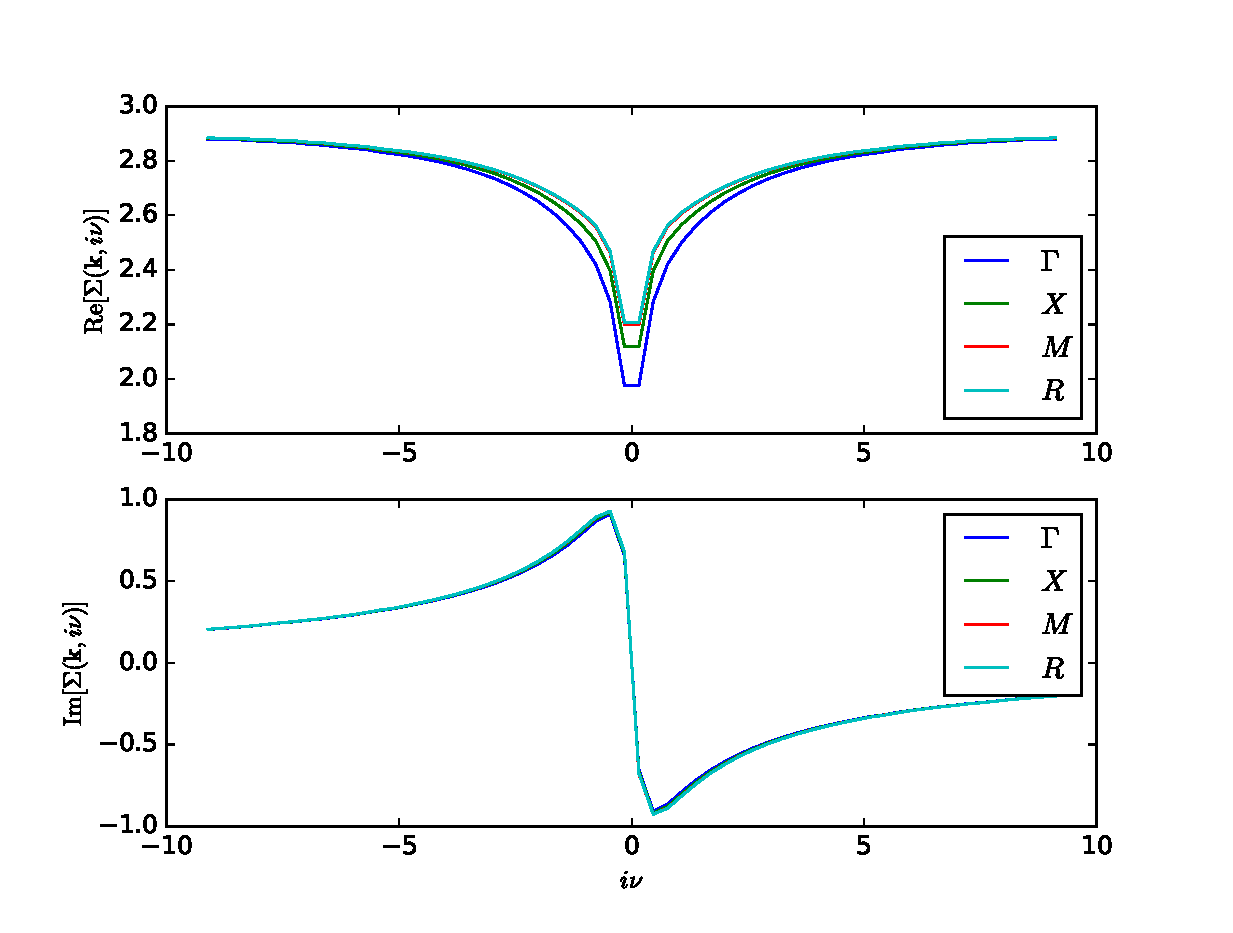
\includegraphics[scale=0.75]{qgrid.eps}
\caption{Selfenergy results for a q-qrid calculation evaluated at high symmetry points. The plot script can be found in {\color{blue}\protect\Verb+/documentation/scripts/1D\_plot\_selfenergy.py+}}
\end{center}
\end{figure}

\begin{figure}[H]
\begin{center}
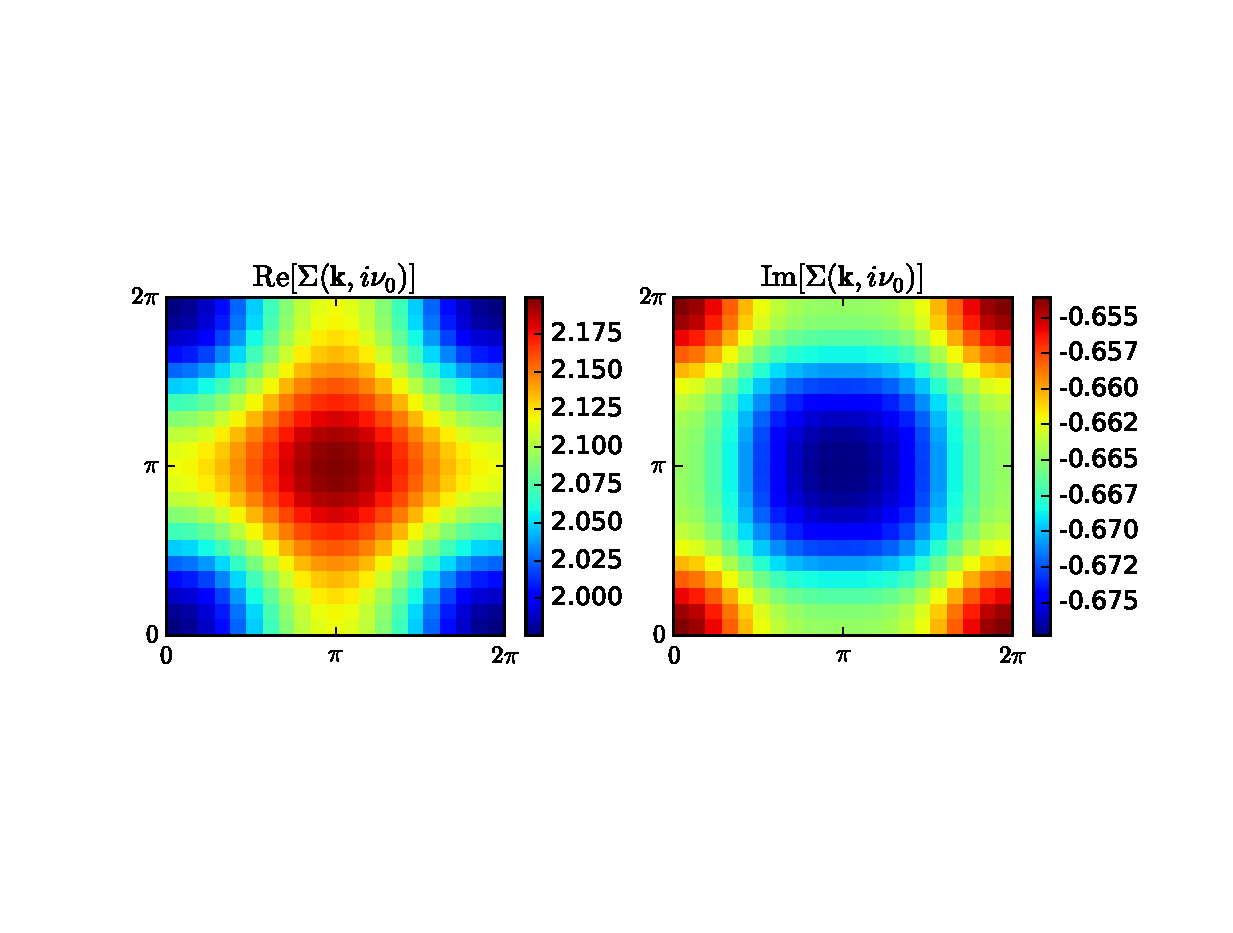
\includegraphics[clip, trim=0cm 3cm 0cm 3cm, scale=0.75]{qgrid_plane.eps}
\caption{Selfenergy results for a q-qrid calculation in the $k_z=0$ plane. Please note that the $\Gamma$ point is located at the bottom left corner. The plot script can be found in {\color{blue}\protect\Verb+/documentation/scripts/2D\_plot\_selfenergy\_plane.py+}}
\end{center}
\end{figure}

\newpage

\begin{figure}[H]
\begin{center}
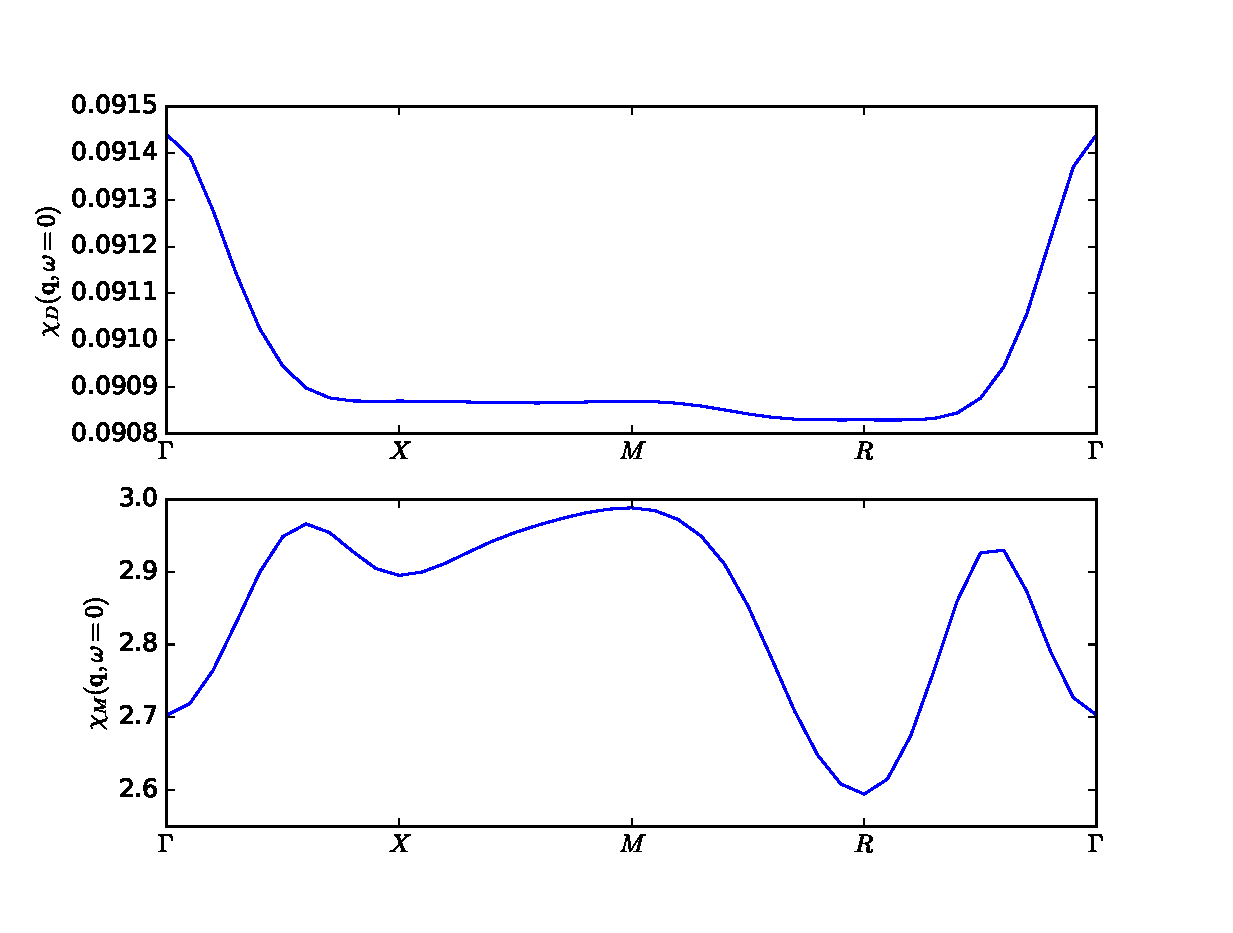
\includegraphics[scale=0.75]{qpath.eps}
\caption{Susceptibility results for a q-path calculation. Please note that a prefactor of 2 is necessary to get the actual magnetic susceptibility. The plot script can be found in {\color{blue}\protect\Verb+/documentation/scripts/1D\_plot\_qpath.py+}}
\end{center}
\end{figure}

Please note that these results are not identical to the ones found in \href{https://arxiv.org/abs/1710.06651}{arXiv:1710.06651}, where we used much larger box sizes in combination with asymptotic vertex behaviour.

\end{document}
